\chapter{पादप अनुकूलन और लक्षणप्ररूपी सुनम्यता}\label{ch:b2:plant-plasticity}

एक ही बलूत की दो पत्तियाँ: मुकुट की चोटी वाली छोटी, मोटी और चमड़े जैसी
है, और छायादार भीतरी भाग वाली उससे तीन गुना बड़ी तथा काग़ज़ जैसी पतली।
उसी बलूत का कोई अंकुर किसी बंद छत्र के नीचे लंबा और दुबला उगता है; और
किसी खुली जगह में उसका सगा छोटा तथा मोटा रह जाता है। इनमें से कोई भी भेद
आनुवंशिक नहीं है। कोई पौधा किसी बेहतर जगह चल नहीं सकता, इसलिए वह स्वयं को
उसी जगह के अनुरूप गढ़ लेता है जो उसे मिली है: वह प्रकाश, गुरुत्व, स्पर्श,
जल, लवण, ठंड भाँपता है, और उसी के अनुसार झुकता, मोटा होता, लंबा होता है,
अपने छिद्र बंद करता है या अपनी कोशिकाएँ कड़ी कर लेता है। यह अध्याय उसी
सुनम्यता के बारे में है --- कि कोई पौधा अपना परिवेश कैसे पढ़ता है और उसके
बारे में क्या करता है --- और उन वंशागत \omterm{def:b2:plant-plasticity:plasticity}{अनुकूलनों} के बारे में
जिनसे वंशक्रमों ने स्वयं को रेगिस्तानों, छाया, लवण और पाले के अनुरूप ढाला है।

\section{सुनम्यता और उसकी सीमाएँ}

\begin{definition}[लक्षणप्ररूपी सुनम्यता और अनुक्रिया-मानक]\label{def:b2:plant-plasticity:plasticity}
\index{लक्षणप्ररूपी सुनम्यता}\index{अनुक्रिया-मानक}\index{अभ्यस्तीकरण}\index{अनुकूलन}
\emph{लक्षणप्ररूपी सुनम्यता} किसी एक \omterm{def:b2:meiosis-heredity:vocabulary}{जीन-प्ररूप} की वह क्षमता है कि वह
भिन्न पर्यावरणों में भिन्न \omterm{def:b2:meiosis-heredity:vocabulary}{लक्षण-प्ररूप} बनाए। किसी \omterm{def:b2:meiosis-heredity:vocabulary}{जीन-प्ररूप} का
\emph{अनुक्रिया-मानक} किसी पर्यावरणीय चर के सापेक्ष उसके \omterm{def:b2:meiosis-heredity:vocabulary}{लक्षण-प्ररूप} का
वक्र है --- प्रकाश के सापेक्ष पत्ती की मोटाई, ताप के सापेक्ष तने की
लंबाई; और \omterm{def:b2:meiosis-heredity:vocabulary}{जीन-प्ररूप} अपने मानकों में भिन्न होते हैं,
तथा वे भेद तब भी वंशागत हैं जब स्वयं वह सुनम्यता न हो।
\emph{अभ्यस्तीकरण} उसका प्रतिवर्ती, शरीरक्रियात्मक रूप है:
कोई पत्ती जो किसी सूखे सप्ताह में अपना उपचर्म मोटा कर ले, या कोई कोशिका
जो शरद में हिमरोधी बनाए। विकास के अर्थ में \emph{अनुकूलन}
किसी वंशक्रम का अपने आवास से वह वंशागत मेल है जो पीढ़ियों में
वरित हुआ; कोई कैक्टस सूखे के लिए अनुकूलित है, और कोई सेम किसी
सूखे दौर से अभ्यस्त होती है। पौधे प्राणियों से अधिक सुनम्य हैं क्योंकि वे
खंडीय और अनिश्चित हैं (\cref{ch:b2:plant-meristems}): अगली
पत्ती पिछली से भिन्न गढ़ी जा सकती है, और स्थिर जीवन
सुनम्यता को चलने का एकमात्र रास्ता बना देता है।
\end{definition}

\begin{omfigure}
\begin{tikzpicture}
\begin{axis}[
  width=0.72\linewidth, height=5.4cm,
  axis x line=bottom, axis y line=left,
  xmin=0, xmax=100, ymin=0, ymax=1.2,
  xlabel={प्रकाश (पूर्ण धूप का \%)}, ylabel={पत्ती की मोटाई (सापेक्ष)},
  xlabel style={font=\small, at={(axis description cs:0.5,-0.13)}, anchor=north},
  ylabel style={font=\small},
  tick label style={font=\small}, xtick={0,25,50,75,100}, ytick={0,0.5,1},
  legend style={font=\scriptsize, at={(0.97,0.08)}, anchor=south east, draw=none},
  clip=false,
]
\addplot[very thick, omDef, domain=2:100, samples=60] {0.35 + 0.65*(1-exp(-x/30))};
\addlegendentry{जीन-प्ररूप 1: कोई सुनम्य बलूत}
\addplot[very thick, omThm, domain=2:100, samples=60] {0.55 + 0.2*(1-exp(-x/30))};
\addlegendentry{जीन-प्ररूप 2: कोई कम सुनम्य बलूत}
\end{axis}
\end{tikzpicture}

{\small दो \omterm{def:b2:plant-plasticity:plasticity}{अनुक्रिया-मानक}। हर \omterm{def:b2:meiosis-heredity:vocabulary}{जीन-प्ररूप} अधिक प्रकाश में मोटी
पत्तियाँ बनाता है; उस वक्र का ढाल --- यानी सुनम्यता --- स्वयं एक
वंशागत लक्षण है, और दोनों \omterm{def:b2:meiosis-heredity:vocabulary}{जीन-प्ररूप} उसमें भिन्न हैं।}
\end{omfigure}

\begin{proposition}[धूप-पत्तियाँ और छाँव-पत्तियाँ]\label{prop:b2:plant-plasticity:sunshade}
\index{धूप-पत्ती}\index{छाँव-पत्ती}
पूर्ण धूप में विकसित होती कोई पत्ती छोटी, मोटी, दो या तीन परतों की
खंभ कोशिकाओं वाली होती है, जिसमें बहुत रंध्र, मोटा उपचर्म,
कार्बन स्थिर करने वाले एंजाइम की ऊँची सांद्रता और
प्रकाशसंश्लेषण की ऊँची अधिकतम दर होती है; जबकि उसी पौधे की छाया में
विकसित होती पत्ती बड़ी, पतली, एक ही खंभ-परत वाली होती है, जिसमें प्रति
इकाई द्रव्यमान अधिक पर्णहरित, कम श्वसन दर और नीचा प्रकाश-प्रतिपूरण
बिंदु होता है। \omterm{prop:b2:plant-plasticity:sunshade}{छाँव-पत्ती} हर फ़ोटॉन को न्यूनतम लागत पर बटोरने के लिए बनी
है, और \omterm{prop:b2:plant-plasticity:sunshade}{धूप-पत्ती} फ़ोटॉनों की बाढ़ को बिना गरमाए या मुरझाए काम में लेने के
लिए। वह निर्णय तब लिया जाता है जब वह पत्ती अब भी प्राथमिकांग है, और उस
प्रकाश से --- विशेषकर उसके रंग से --- जो उस कलिका तक पहुँचे;
कोई परिपक्व पत्ती स्वयं को फिर नहीं गढ़ सकती, और इसीलिए छाया से धूप में
ले जाया गया कोई पौधा तब तक झुलसता है जब तक वह नई पत्तियाँ न बना ले।
\end{proposition}

\begin{omfigure}
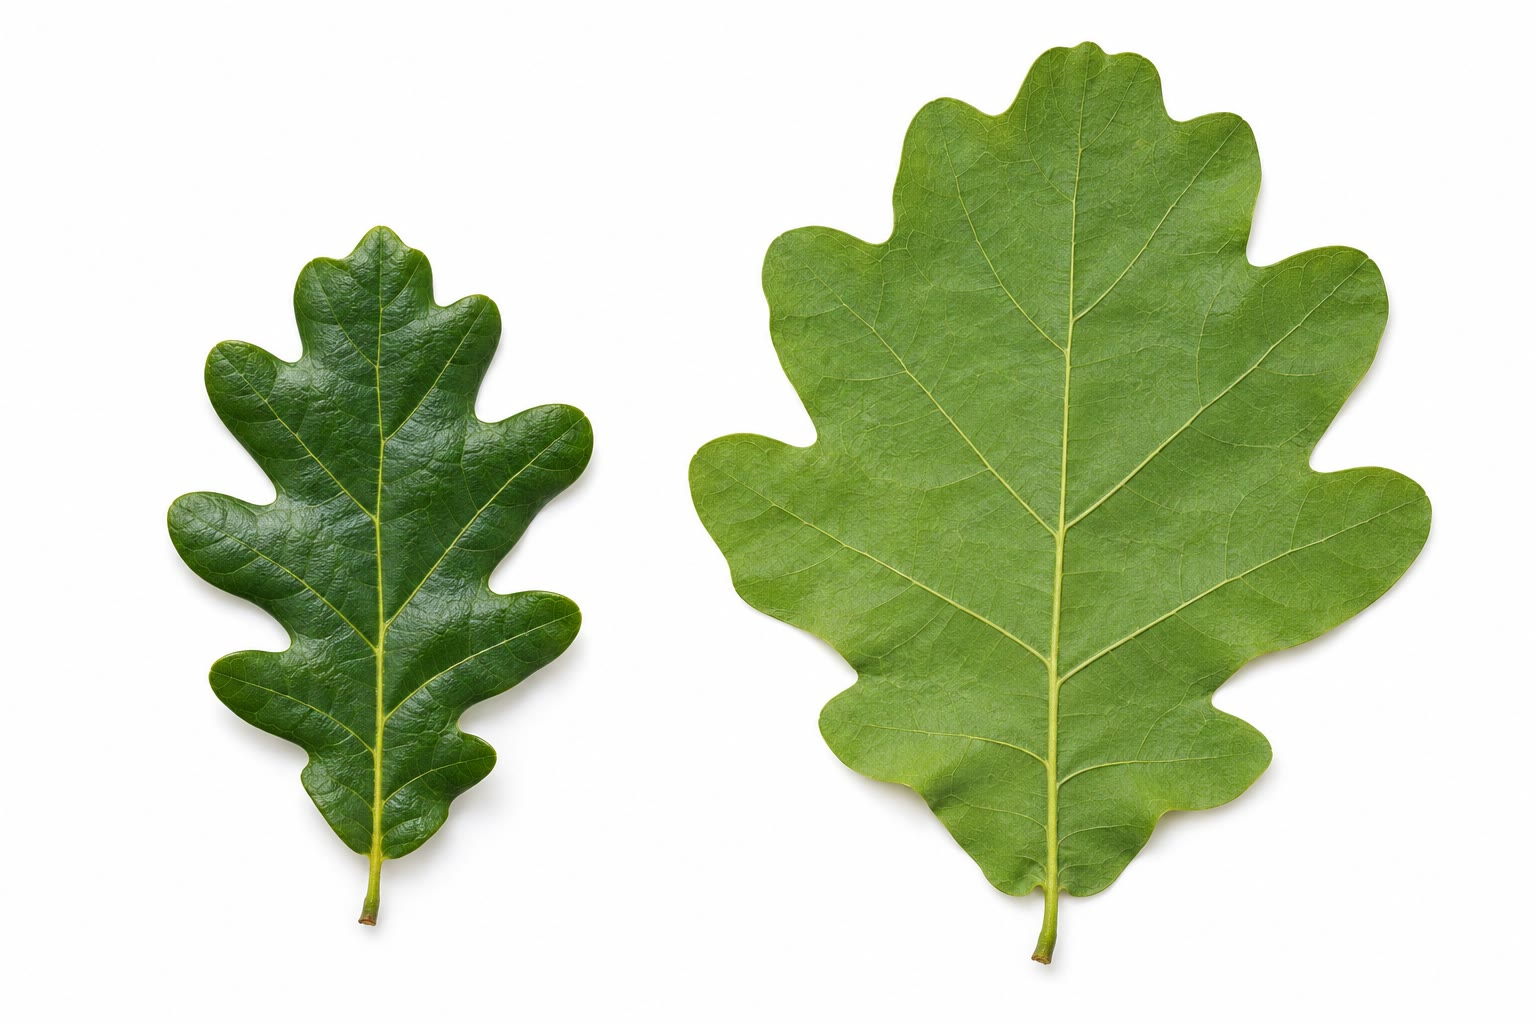
\includegraphics[width=0.55\linewidth]{images/book4/ai/b4-15-sun-shade-leaves.jpg}

{\small एक ही बलूत की एक \omterm{prop:b2:plant-plasticity:sunshade}{धूप-पत्ती} और एक \omterm{prop:b2:plant-plasticity:sunshade}{छाँव-पत्ती}: वही \omterm{def:b2:meiosis-heredity:vocabulary}{जीन-प्ररूप},
भिन्न प्रकाश, भिन्न पत्तियाँ।}
\end{omfigure}

\section{प्रकाश पढ़ना}

\begin{theorem}[प्रकाश-गुण के मापी के रूप में फ़ाइटोक्रोम]\label{thm:b2:plant-plasticity:phytochrome}
\index{फ़ाइटोक्रोम}\index{लाल:दूर-लाल अनुपात}\index{छाया-परिहार}
फ़ाइटोक्रोम दो रूपों में है: $P_r$, जो लाल प्रकाश
(\qty{660}{nm}) अवशोषित करता है और $P_{fr}$ में बदल जाता है, और $P_{fr}$, जो
दूर-लाल (\qty{730}{nm}) अवशोषित करता है और वापस बदल जाता है --- और काम
$P_{fr}$ ही करता है। सतत प्रकाश में वे दोनों रूपांतरण किसी
\emph{प्रकाश-साम्य} पर संतुलित होते हैं, जिसकी स्थिति केवल प्रकाश में
लाल और दूर-लाल के अनुपात पर निर्भर है:
\[
\varphi = \frac{P_{fr}}{P_{r} + P_{fr}} = \frac{R}{R + a\,FR},
\]
जिसमें $R$ और $FR$ दोनों पट्टियों में फ़ोटॉन अभिवाह-घनत्व हैं
और $a$ उस रंजक का एक स्थिरांक ($a \approx 0.77$)। सूर्य-प्रकाश में
$R{:}FR \approx 1.15$ है, जो $\varphi \approx 0.6$ देता है; जबकि
पत्तियों से छना प्रकाश, जो लाल अवशोषित करती और दूर-लाल संचारित करती हैं, $R{:}FR
\approx 0.2$ और $\varphi \approx 0.2$ रखता है। नीचा $\varphi$ किसी
पौधे को बता देता है कि वह दूसरे पौधों के नीचे या बग़ल है, और वह भी असल
में छाया पड़ने से पहले --- किसी पड़ोसी से परावर्तित दूर-लाल उसी ओर की सतह
पर पकड़ा जाता है --- और वह \emph{\omterm{thm:b2:plant-plasticity:phytochrome}{छाया-परिहार} संलक्षण} से उत्तर देता है:
तेज़ तना-दीर्घीकरण, लंबे वृंत, ऊपर उठी पत्तियाँ, कम शाखन, और जल्दी
पुष्पन। किसी बंद छत्र में कोई अंकुर अपने दीर्घीकरण की दर दुगुनी कर लेता है।
\end{theorem}
\begin{proof}
मान लीजिए $k_1 R$ $P_r \to P_{fr}$ का दर-नियतांक है (जो लाल अभिवाह के
समानुपाती है) और $k_2\,FR$ $P_{fr} \to P_r$ का। साम्य पर
$k_1 R\,P_r = k_2\,FR\,P_{fr}$, इसलिए $P_{fr}/P_r = k_1 R/
(k_2 FR)$ और $\varphi = P_{fr}/(P_r + P_{fr}) = R/(R + a\,FR)$, जिसमें
$a = k_2/k_1$। (दोनों रूप दोनों पट्टियों में कुछ-कुछ अवशोषित करते हैं,
जिसे वह स्थिरांक $a$ समेट लेता है; परिणाम का रूप वही रहता है।)
$a = 0.77$ के साथ: $1.15/(1.15 + 0.77) = 0.60$; $0.2/(0.2 + 0.77) = 0.21$।
\end{proof}

\begin{omfigure}
\begin{tikzpicture}
\begin{axis}[
  width=0.7\linewidth, height=5.2cm,
  axis x line=bottom, axis y line=left,
  xmin=0, xmax=1.4, ymin=0, ymax=0.8,
  xlabel={प्रकाश का लाल : दूर-लाल अनुपात}, ylabel={$\varphi = P_{fr}/P_{\text{कुल}}$},
  xlabel style={font=\small, at={(axis description cs:0.5,-0.13)}, anchor=north},
  ylabel style={font=\small},
  tick label style={font=\small}, xtick={0,0.2,0.6,1.15}, ytick={0,0.2,0.4,0.6},
  clip=false,
]
\addplot[very thick, omDef, domain=0:1.4, samples=60] {x/(x+0.77)};
\draw[dashed, gray] (axis cs:1.15,0) -- (axis cs:1.15,0.6) -- (axis cs:0,0.6); \node[font=\scriptsize, anchor=south west] at (axis cs:1.15,0.6) {खुली धूप};
\draw[dashed, gray] (axis cs:0.2,0) -- (axis cs:0.2,0.21) -- (axis cs:0,0.21); \node[font=\scriptsize, anchor=west] at (axis cs:0.25,0.15) {किसी छत्र के नीचे};
\end{axis}
\end{tikzpicture}

{\small लाल-से-दूर-लाल अनुपात के सापेक्ष फ़ाइटोक्रोम का प्रकाश-साम्य।
सूर्य-प्रकाश उस रंजक का अधिकांश सक्रिय रूप में रखता है; जबकि
पत्ती-छना प्रकाश उसे अधिकतर निष्क्रिय रखता है, और वह पौधा
उस भेद को पड़ोसियों के रूप में पढ़ता है।}
\end{omfigure}

\begin{proposition}[प्रकाशानुवर्तन]\label{prop:b2:plant-plasticity:phototropism}
\index{प्रकाशानुवर्तन}\index{अनुवर्तन}\index{कोलोदनी--वेंट परिकल्पना}
\emph{अनुवर्तन} किसी दिशात्मक उद्दीपन से अभिविन्यस्त वृद्धि-गति है।
\emph{प्रकाशानुवर्तन} में कोई प्ररोह नीले प्रकाश की ओर झुकता है:
उस प्रकाश को सिरे पर कोई नील-प्रकाश ग्राही
(फ़ोटोट्रोपिन) भाँपता है, सिरे से उतरती ऑक्सिन छायादार भाग की ओर मोड़ दी
जाती है --- उसके वाहक पार्श्व झिल्ली पर चले जाते हैं ---
और छायादार भाग, अधिक ऑक्सिन पाकर, प्रकाशित भाग से तेज़ लंबा होता है,
इसलिए वह प्ररोह प्रकाश की ओर मुड़ जाता है। वह
झुकाव अवकल वृद्धि है, कोई पेशी नहीं: वह केवल
\omterm{prop:b2:plant-meristems:ram}{दीर्घीकरण क्षेत्र} में होता है, उसमें एक-दो घंटे लगते हैं, और वह अप्रतिवर्ती है।
जड़ों में, जहाँ वही ऑक्सिन-आधिक्य दीर्घीकरण को \emph{संदमित} करता है, वे
दूर झुकती हैं।
\end{proposition}
\begin{proof}[प्रमाण-सामग्री]
डार्विन (1880) ने घास के प्रांकुर-चोलों से दिखाया कि सिरा उस
प्रकाश को भाँपता है और उसके नीचे का क्षेत्र झुकता है:
सिरे को किसी अपारदर्शी टोपी से ढकने पर वह झुकाव मिट गया, आधार को किसी
नली से ढकने पर नहीं, और किसी पारदर्शी टोपी ने उसे अक्षत छोड़ दिया।
बोयसन-येन्सन (1913) ने सिरा काटकर उसे बीच में जिलेटिन के एक खंड के साथ
वापस रख दिया: झुकाव बना रहा, इसलिए वह संकेत कोई विसरणशील पदार्थ था; और
अभ्रक की एक पत्ती छायादार भाग में डालने से वह रुक गया, प्रकाशित भाग में
डालने से नहीं, इसलिए वह पदार्थ छायादार भाग से नीचे उतरता था। वेंट (1928)
ने कटे सिरों से वह पदार्थ अगार में इकट्ठा किया और पाया कि अँधेरे में
किसी शीर्ष-रहित प्रांकुर-चोल पर केंद्र से हटकर रखा गया खंड उसे उस खंड से
दूर झुका देता था --- और वह भी उस मात्रा के समानुपाती कोण से ---
तथा एकपार्श्व प्रकाशित सिरे के दोनों आधे भागों से अगार इकट्ठा करके
उन्होंने ऑक्सिन का लगभग दो तिहाई छायादार भाग में और एक तिहाई
प्रकाशित भाग में पाया (ब्रिग्स, 1957, बेहतर विधियों से)। किसी वृद्धि
हॉर्मोन का यही पार्श्व पुनर्वितरण \omterm{prop:b2:plant-plasticity:phototropism}{कोलोदनी--वेंट
परिकल्पना} है, और वह टिकी हुई है।
\end{proof}

\begin{omfigure}
\begin{tikzpicture}[every node/.style={font=\scriptsize}, >=stealth]
  \foreach \x/\lab/\cap/\bend in {0/{अक्षत:\\झुकता है}/0/1, 2.6/{सिरा ढका:\\नहीं झुकता}/1/0, 5.2/{आधार ढका:\\झुकता है}/2/1, 7.8/{सिरा कटा:\\नहीं झुकता}/3/0, 10.4/{सिरा जिलेटिन पर:\\झुकता है}/4/1} {
    \begin{scope}[xshift=\x cm]
      \fill[omExo!30] (-0.7,0) rectangle (0.7,0.2);
      \ifnum\bend=1
        \draw[very thick, omExo!70!black] (0,0.2) -- (0,1.6) .. controls (0,2.3) and (0.5,2.6) .. (0.9,2.8);
      \else
        \draw[very thick, omExo!70!black] (0,0.2) -- (0,3.0);
      \fi
      \ifnum\cap=1 \fill[black] (-0.2,2.7) rectangle (0.2,3.1); \fi
      \ifnum\cap=2 \fill[black] (-0.2,0.2) rectangle (0.2,1.5); \fi
      \ifnum\cap=3 \draw[thick] (-0.3,2.6) -- (0.3,2.6); \fi
      \ifnum\cap=4 \fill[omDef!35] (-0.2,2.55) rectangle (0.2,2.75); \draw[very thick, omExo!70!black] (0.55,2.75) -- (0.9,3.1); \fi
      \node[below, align=center] at (0,-0.15) {\lab};
    \end{scope}
  }
  \node[anchor=east, align=right, omProp!80!black] at (-1.0,2.2) {दाईं ओर से\\प्रकाश $\to$};
\end{tikzpicture}

{\small प्रांकुर-चोल के प्रयोग। डार्विन: सिरा उस प्रकाश को
भाँपता है और नीचे का क्षेत्र झुकता है; सिरा ढकने से वह रुक जाता है,
आधार ढकने से नहीं। बोयसन-येन्सन: वह संकेत जिलेटिन के किसी खंड को पार कर
जाता है --- यानी वह कोई पदार्थ है।}
\end{omfigure}

\begin{omfigure}
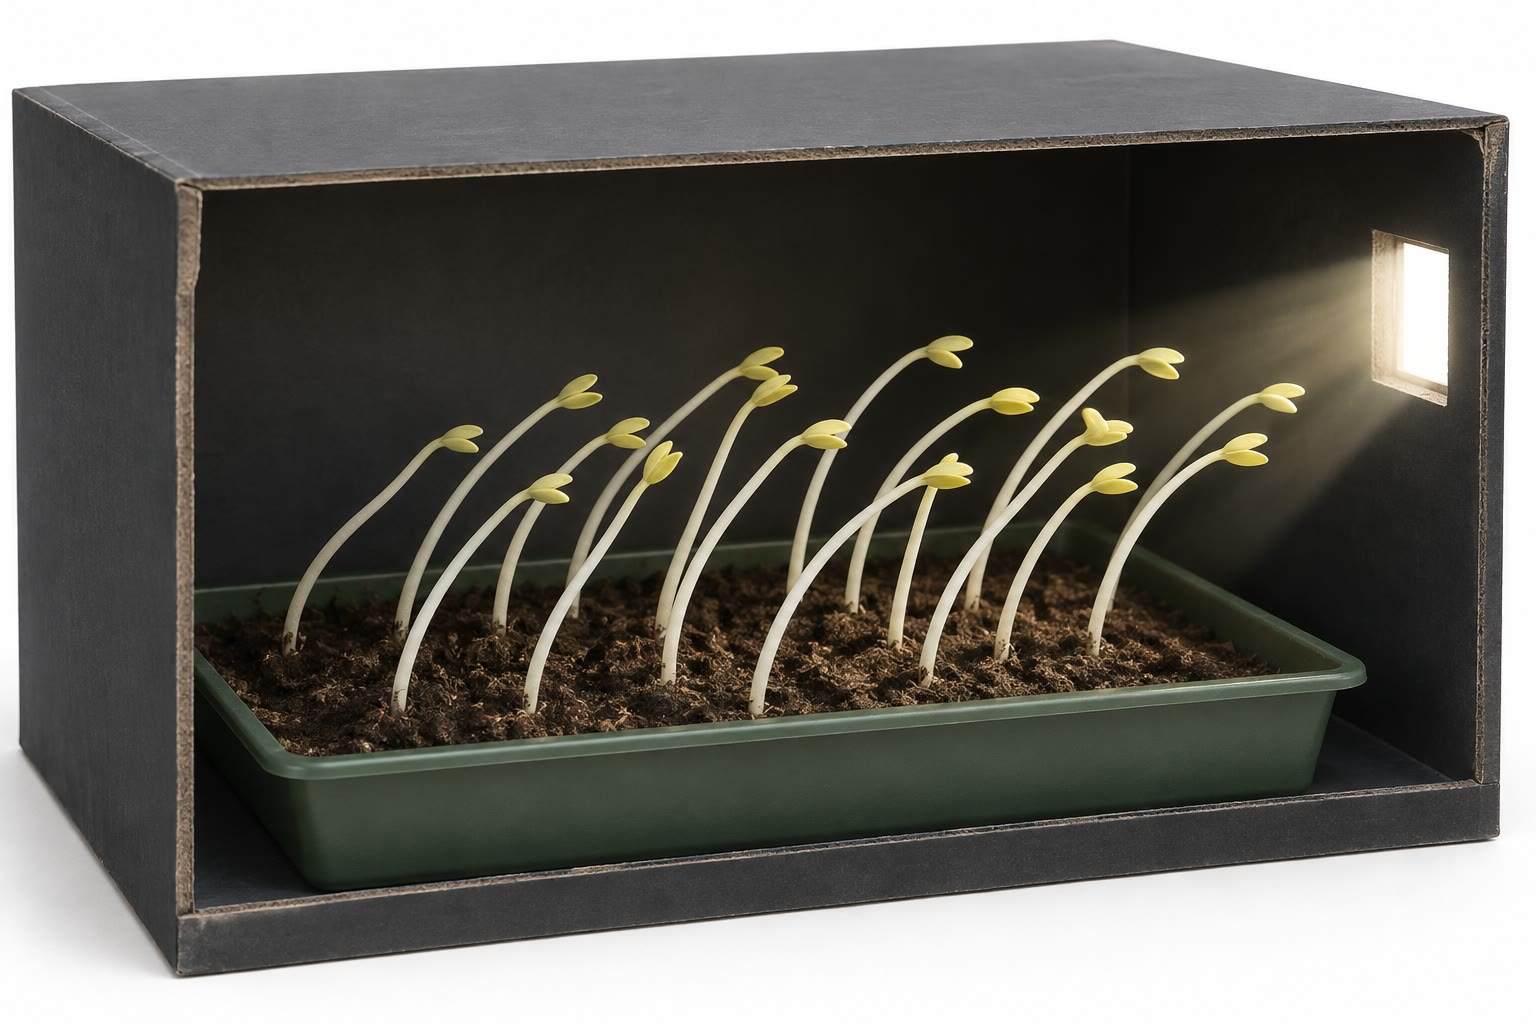
\includegraphics[width=0.55\linewidth]{images/book4/ai/b4-15-phototropism.jpg}

{\small एक ही खिड़की वाले किसी डिब्बे में अंकुर: सब उस प्रकाश की ओर
झुकते हैं, और वह भी उससे दूर वाले भाग में तेज़ बढ़कर।}
\end{omfigure}

\begin{theorem}[कोई तना कितना झुकता है]\label{thm:b2:plant-plasticity:bend}
यदि $d$ व्यास के किसी तने का छायादार भाग सापेक्ष मात्रा
$\varepsilon_s$ से और प्रकाशित भाग $\varepsilon_l$ से, $L$ लंबाई के किसी
वृद्धि-क्षेत्र पर, लंबा हो, तो वह क्षेत्र इस कोण से मुड़ता है:
\[
\theta = \frac{L\,(\varepsilon_s - \varepsilon_l)}{d}
\]
(रेडियन में)। \qty{10}{mm} के क्षेत्र पर घंटे भर में \qty{5}{\%} बढ़ता
और \qty{1}{mm} चौड़ा कोई प्रांकुर-चोल, जिसमें ऑक्सिन
$65 : 35$ बँटी हो ताकि दोनों भाग माध्य के $1.3$ और $0.7$ गुना बढ़ें,
तीन घंटों में $\theta = 10\times(0.195 - 0.105)/1 =
0.9$ रेडियन, यानी लगभग \qty{50}{\degree}, झुक जाता है। झुकने को कोई नई
क्रियाविधि नहीं चाहिए: \cref{ch:b2:plant-meristems} की साधारण वृद्धि,
दोनों भागों पर असमान कर दी जाए, पर्याप्त है।
\end{theorem}
\begin{proof}
उस क्षेत्र के दोनों भाग $\rho + d/2$ और $\rho - d/2$ त्रिज्याओं के ऐसे
चाप बन जाते हैं जो वही कोण $\theta$ अंतरित करते हैं, और जिनकी लंबाइयाँ $L(1 +
\varepsilon_s)$ तथा $L(1 + \varepsilon_l)$ हैं; उनका अंतर
$\theta d$ है, इसलिए $\theta = L(\varepsilon_s - \varepsilon_l)/d$। घंटे
भर में \qty{5}{\%} की दर से तीन घंटों में माध्य विस्तार $0.15$ है;
और $1.3\times 0.15 = 0.195$ तथा $0.7\times 0.15 = 0.105$।
\end{proof}

\begin{proposition}[गुरुत्वानुवर्तन]\label{prop:b2:plant-plasticity:gravitropism}
\index{गुरुत्वानुवर्तन}\index{स्टैटोलिथ}
बग़ल में लिटाया गया कोई प्ररोह घंटों में ऊपर की ओर मुड़ जाता है और कोई
जड़ नीचे की ओर। गुरुत्व की दिशा \emph{स्टैटोलिथ} भाँपते हैं ---
यानी \omterm{prop:b2:plant-meristems:ram}{मूल टोप} की और तने के मंड-आवरण की विशिष्ट कोशिकाओं के
घने मंड-कण --- जो सेकंडों में उस कोशिका के निचले भाग में बैठ जाते हैं
और, झिल्ली या अंतर्द्रव्यी जालिका पर दबाव डालकर, ऑक्सिन के वाहक इस तरह
मोड़ देते हैं कि ऑक्सिन निचले भाग में जमा हो जाए। प्ररोह में निचला भाग
तेज़ बढ़ता है और वह तना ऊपर मुड़ जाता है; जबकि जड़ में वही ऑक्सिन-आधिक्य
निचले भाग को संदमित करता है, ऊपरी भाग तेज़ बढ़ता है, और वह जड़ नीचे मुड़
जाती है। \omterm{prop:b2:plant-meristems:ram}{मूल टोप} हटा दीजिए और वह जड़ किसी भी दिशा में सीधी बढ़ती है;
मंड-रहित उत्परिवर्ती गुरुत्व ठीक से नहीं भाँपते; और किसी धीरे घूमते ढोल
(क्लाइनोस्टेट) पर रखी जड़, जो उन स्टैटोलिथों को कभी बैठने ही नहीं देता,
बिना किसी दिशा के बढ़ती है। यह अनुक्रिया उसी
कोलोदनी--वेंट क्रियाविधि का दूसरा उपयोग है, पर भिन्न संवेदक के साथ।
\end{proposition}

\section{जल: छिद्र बंद करना}

\begin{proposition}[रंध्रीय नियंत्रण]\label{prop:b2:plant-plasticity:stomata}
\index{रंध्र}\index{द्वार कोशिका}\index{ऐब्सिसिक अम्ल}\index{रंध्रीय चालकता}
पत्ती के छिद्र, यानी \emph{रंध्र}, हर एक दो
\emph{\omterm{prop:b2:plant-plasticity:stomata}{द्वार कोशिकाओं}} से घिरे हैं जिनकी भित्तियाँ असमान रूप से मोटी हैं,
इसलिए जब वे पोटैशियम तथा जल लेकर फूलती हैं तब वे अलग होकर वह छिद्र खोल
देती हैं, और जब वे उन्हें खो देती हैं तब उसे बंद कर देती हैं। वे सुबह
नीले प्रकाश में और नीची भीतरी $\mathrm{CO_2}$ पर खुलती हैं, और
अँधेरे में बंद हो जाती हैं; और वे मिनटों में बंद हो जाती हैं जब
\emph{\omterm{def:b2:plant-flowering:dormancy}{ऐब्सिसिक अम्ल}} आ पहुँचे --- जो सूखती मिट्टी भाँपती जड़ों में बनता
है और जाइलम में ऊपर ढोया जाता है, या स्वयं उस पत्ती में बनता है जब वह
स्फीति खोए --- और तब भी जब वायु बहुत शुष्क हो। \emph{\omterm{prop:b2:plant-plasticity:stomata}{रंध्रीय चालकता}}
$g_s$ दोनों तय करती है: खोया जाता जल, $E = g_s\,(w_i - w_a)$ (यानी
पत्ती के संतृप्त भीतरी भाग और वायु के बीच जलवाष्प के मोल-अंश का अंतर),
और भीतर लिया जाता $\mathrm{CO_2}$, $A = g_s\,(c_a -
c_i)/1.6$ (जिसमें गुणक $1.6$ जलवाष्प और $\mathrm{CO_2}$ की विसरणशीलताओं
का अनुपात है)। वह पत्ती एक ही वाल्व से जल का कार्बन से सौदा करती है,
और उसकी \emph{जल-उपयोग दक्षता} है
\[
\frac{A}{E} = \frac{c_a - c_i}{1.6\,(w_i - w_a)},
\]
यानी प्रति मोल जल कार्बन के कुछ हज़ारवें मोल: कोई प्रारूपिक
C$_3$ पत्ती प्रति ग्राम स्थिर कार्बन \qtyrange{400}{600}{g} जल ख़र्च
करती है, कोई C$_4$ पत्ती उसका आधा, और कोई \omterm{prop:b2:plant-plasticity:xerophytes}{CAM पौधा} पाँचवाँ भाग।
\end{proposition}

\begin{omfigure}
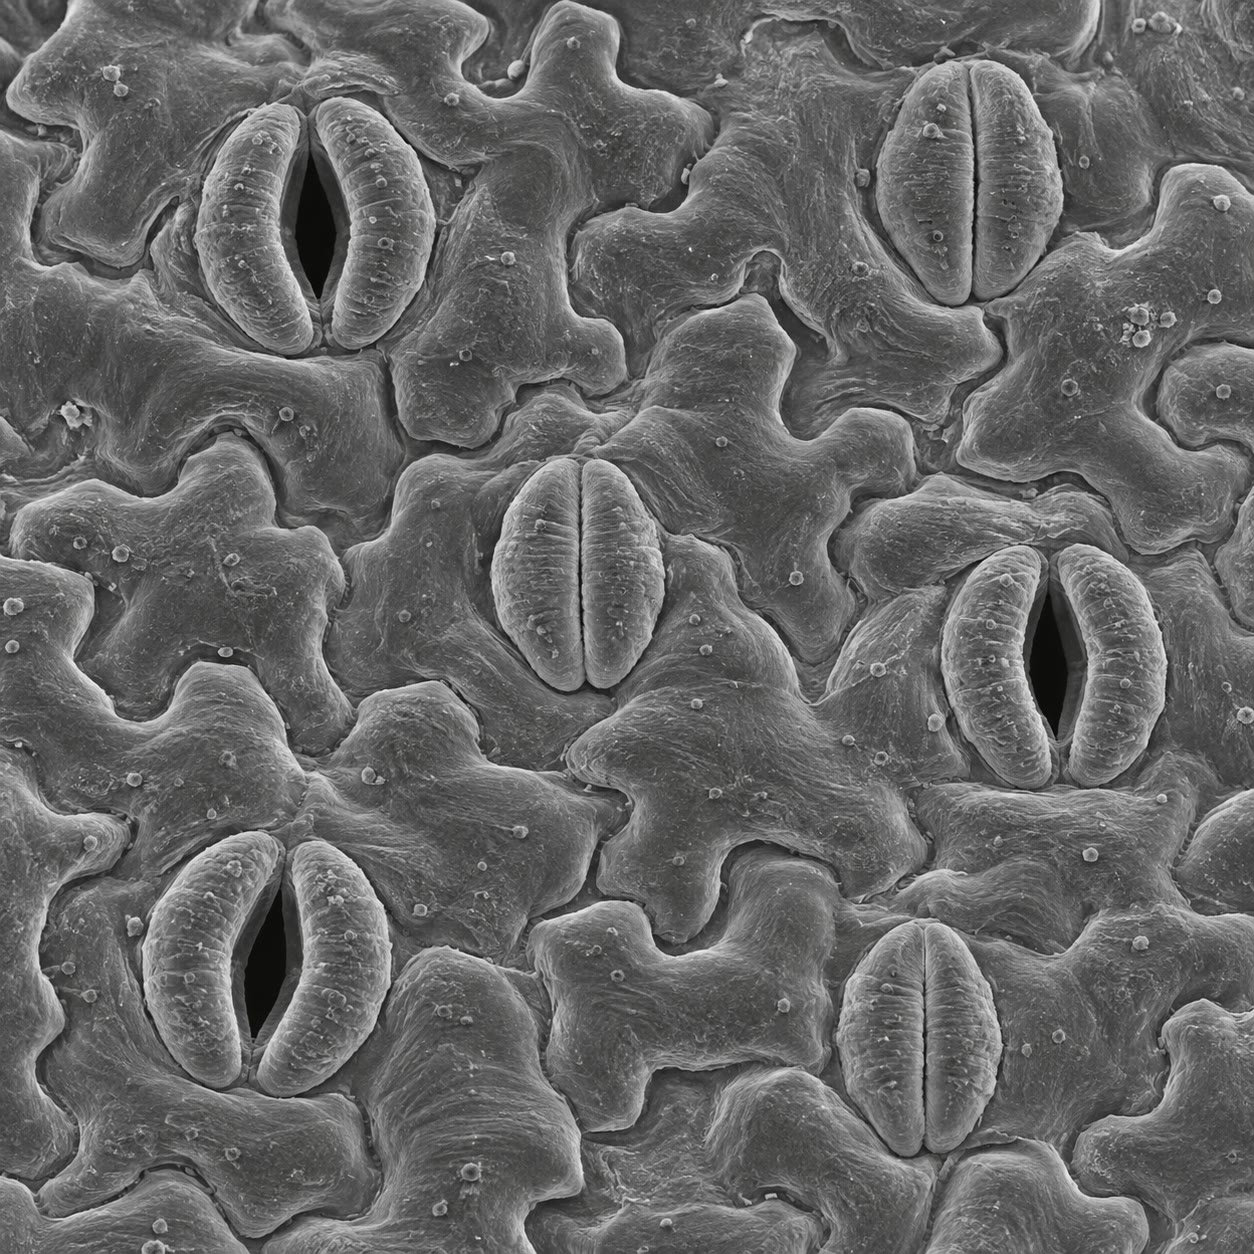
\includegraphics[width=0.42\linewidth]{images/book4/ai/b4-15-stomata-sem.jpg}

{\small किसी पत्ती की निचली सतह पर रंध्र, कुछ खुले और कुछ
बंद: हर छिद्र के चारों ओर दो \omterm{prop:b2:plant-plasticity:stomata}{द्वार कोशिकाएँ}, यानी वही वाल्व जिससे
वह पत्ती जल का कार्बन डाइऑक्साइड से सौदा करती है।}
\end{omfigure}

\begin{example}[एक दिन के कार्बन की क़ीमत]\label{ex:b2:plant-plasticity:wue}
दोपहर में सूरजमुखी की किसी पत्ती में, जिसका $g_s = \qty{0.3}{mol.m^{-2}.s^{-1}}$,
$w_i - w_a = 0.02$ और $c_a - c_i = \qty{120}{\micro mol/mol}$ है,
वाष्पोत्सर्जन $E = \qty{6}{mmol.m^{-2}.s^{-1}}$ होता है और वह $A =
0.3\times 120/1.6 = \qty{22}{\micro mol.m^{-2}.s^{-1}}$ स्थिर करती है: $A/E =
\qty{3.7e-3}{}$, यानी हर कार्बन परमाणु के लिए जल के 270 अणु, यानी
प्रति ग्राम कार्बन \qty{400}{g} जल। ऐसी पत्तियों का एक हेक्टेयर किसी
ग्रीष्म दिन में \qty{100}{kg} कार्बन स्थिर करने के लिए \qty{40}{t} जल
खो देता है। मिट्टी सूखने पर \omterm{def:b2:plant-flowering:dormancy}{ऐब्सिसिक अम्ल} उन रंध्रों को इस चालकता के
दसवें भाग तक बंद कर देता है: $E$ दस गुना गिरता है, $A$ उससे कम
(क्योंकि $c_i$ भी गिरता है), और वह पौधा प्यास से मरने के बजाय भुखमरी की
ख़ुराक पर जी लेता है।
\end{example}

\begin{proposition}[सूखे के अनुकूलन]\label{prop:b2:plant-plasticity:xerophytes}
\index{शुष्कोद्भिद}\index{CAM पौधा}\index{मांसल पौधा}
सूखी जगहों के पौधे (\emph{शुष्कोद्भिद}) वंशागत
संरचनाएँ और रणनीतियाँ मिलाते हैं। हानि घटाइए: मोटा उपचर्म, गड्ढों में
या रोमों के नीचे धँसे रंध्र (जो स्थिर वायु की परत मोटी करते हैं),
काँटों में घटी पत्तियाँ (कैक्टस) या शुष्क ऋतु में झाड़ दी गईं, और छोटी
मोटी पत्तियाँ जो मुड़ जाती हैं। सँजोइए: जल थामने वाले श्लेष्म सहित मांसल
तने और पत्तियाँ। पहुँचिए: \qty{50}{m} गहरी जड़ें (मेसकीट) या सतह के ठीक
नीचे फैली जड़ें जो किसी बौछार को पकड़ लें। बदलिए: CAM
पौधे अपने रंध्र रात में खोलते हैं, जब $w_i - w_a$ छोटा है,
$\mathrm{CO_2}$ को मैलिक अम्ल में स्थिर करते हैं, और दिन में बंद रंध्रों
के पीछे उसे फिर स्थिर करते हैं --- यानी वही कार्बन, पाँचवें भाग जल पर।
भागिए: रेगिस्तानी एकवर्षी वर्षों तक \omterm{def:b2:angiosperm-reproduction:seed}{बीजों} के रूप में जीते हैं और
वर्षा के बाद के सप्ताहों में एक पूरा \omterm{def:b2:plant-life-cycles:cycles}{जीवन-चक्र} पूरा कर लेते हैं।
सहिए: पुनरुज्जीवी पौधे अपना \qty{95}{\%} जल खोकर फिर जी उठते हैं।
हर रणनीति का एक दाम है --- CAM धीमा है, मांसलता भारी है, काँटे
प्रकाशसंश्लेषण नहीं कर सकते --- और जो पौधा वह दाम चुकाता है वह जहाँ भी
जल प्रचुर हो वहाँ पीछे छूट जाता है।
\end{proposition}

\begin{omfigure}
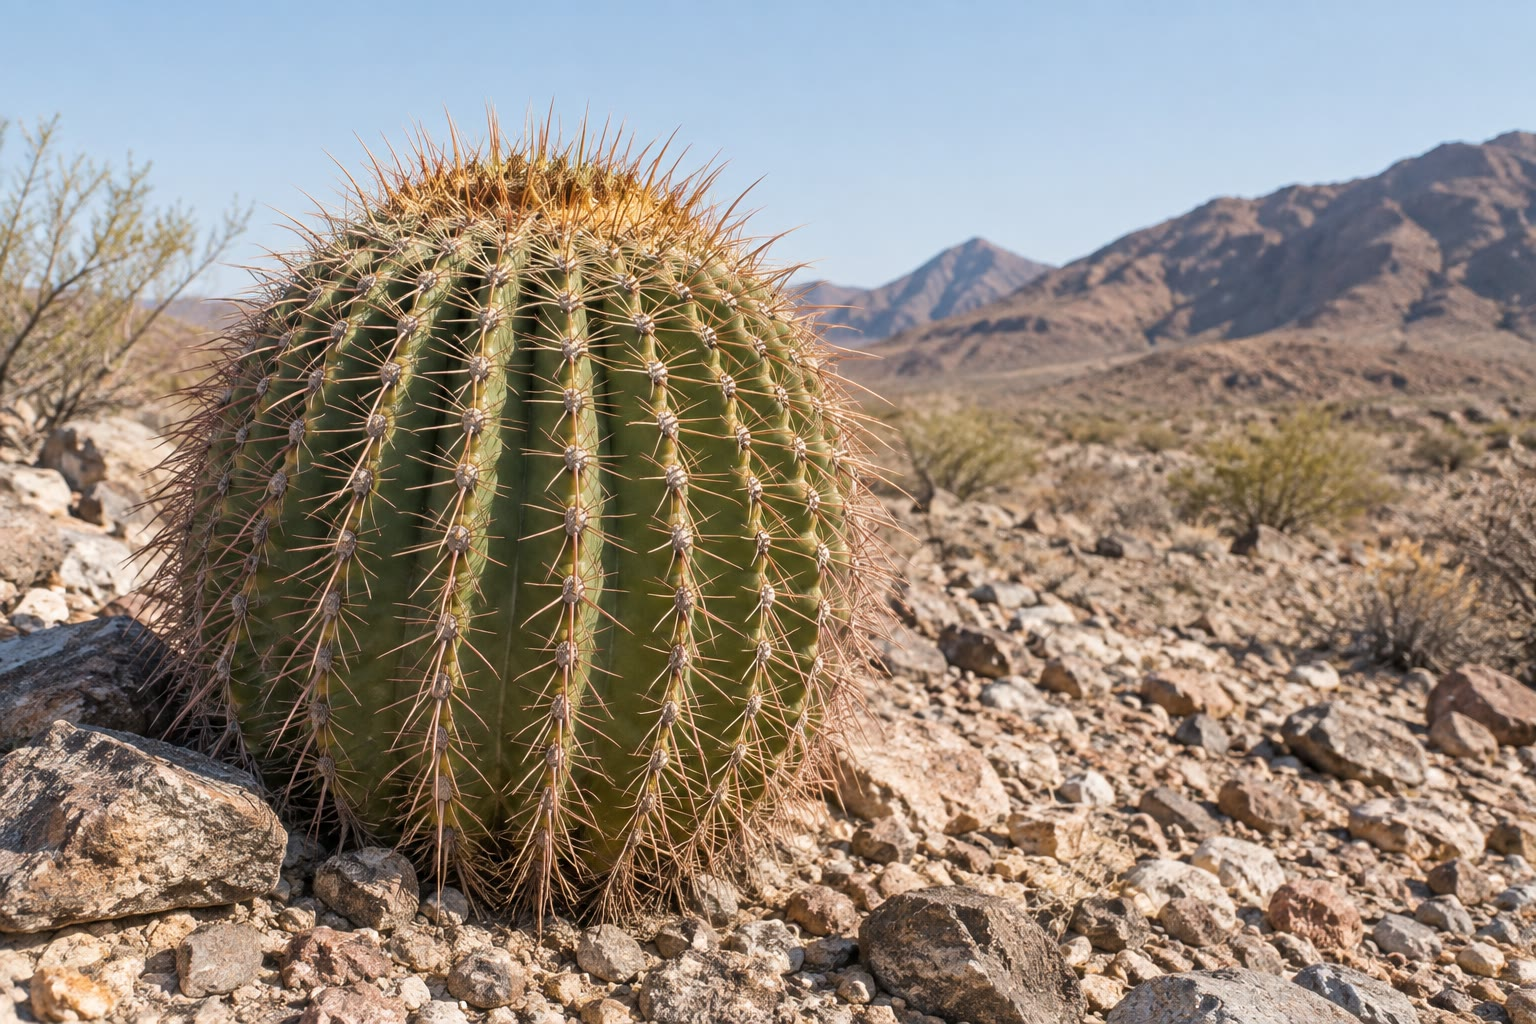
\includegraphics[width=0.55\linewidth]{images/book4/ai/b4-15-cactus.jpg}

{\small कोई पीपा-कैक्टस: मोटे उपचर्म वाला एक मांसल तना,
ऐसी पर्शुकाएँ जो उसे वर्षा के बाद फूलने देती हैं, काँटों में घटी
पत्तियाँ, और ऐसे रंध्र जो केवल रात में खुलते हैं।}
\end{omfigure}

\section{ठंड, लवण और दबाव-अनुक्रिया}

\begin{proposition}[दबाव से अभ्यस्तीकरण]\label{prop:b2:plant-plasticity:stress}
\index{शीत अभ्यस्तीकरण}\index{लवणोद्भिद}\index{ऊष्मा-आघात प्रोटीन}
\qty{4}{\celsius} पर एक सप्ताह उस ताप को, जो किसी शीतकालीन राई को
मार डालता है, \qty{-5}{\celsius} से घटाकर \qty{-25}{\celsius} कर देता
है: उन कोशिकाओं ने ऐसी शर्कराएँ तथा प्रोटीन भर लिए हैं जो हिमांक गिराते
और झिल्लियाँ बचाते हैं, अपने लिपिड बदलकर उन्हें तरल रखा है, और ऐसे
हिमरोधी प्रोटीन बना लिए हैं जो हिम-रवों को बढ़ने से रोकते हैं; और मारक
घटना वह हिम नहीं है, जो कोशिकाओं के बीच निरापद बनती है, बल्कि उस कोशिका
का निर्जलीकरण है जब जल उसे छोड़कर हिम से जा मिलता है। \qty{40}{\celsius} पर कुछ
घंटे \emph{\omterm{prop:b2:plant-plasticity:stress}{ऊष्मा-आघात प्रोटीन}} प्रेरित करते हैं जो
विकृतीकृत प्रोटीन फिर मोड़ देते हैं और उस कोशिका को
\qty{45}{\celsius} पर बचाते हैं। लवण का सामना जड़ पर अपवर्जन से,
रसधानी में डिब्बाबंदी से (और कोशिकाद्रव में उसे संतुलित करने वाले
अनुकूल विलेयों से), और सच्चे \emph{लवणोद्भिदों} में लवण-ग्रंथियों से
स्राव द्वारा किया जाता है। इनमें से अधिकांश अनुक्रियाएँ उसी
संकेतन से गुज़रती हैं: कोई संवेदक, कोशिकाद्रवी कैल्सियम की चढ़ाई,
\omterm{def:b2:plant-flowering:dormancy}{ऐब्सिसिक अम्ल}, और ऐसे \omterm{prop:b2:cell-differentiation:transcriptional}{अनुलेखन कारकों} का एक समुच्चय जो सैकड़ों
रक्षक जीन चालू कर देते हैं --- यानी किसी प्राणी की प्रतिरक्षा अनुक्रिया
जितना ही सामान्य एक दबाव-कार्यक्रम, और उसी की तरह महँगा: अभ्यस्त हुआ
पौधा धीरे बढ़ता है, और जो पौधा बिना ज़रूरत अभ्यस्त हो जाए वह उससे हार
जाता है जो नहीं होता।
\end{proposition}
\begin{proof}[प्रमाण-सामग्री]
शीत-अभ्यस्तीकरण के प्रयोग उस ताप को मापते हैं जिस पर किसी पत्ती की
आधी कोशिकाएँ मर जाती हैं (यानी LT$_{50}$), और वह भी किसी कम ताप की
अवधि से पहले तथा बाद में; और सप्ताह भर में दस से बीस अंश की वह खिसक
सप्ताह भर की गर्मी से उलट जाती है। जो उत्परिवर्ती शीत
कार्यक्रम चालू नहीं कर पाते (CBF \omterm{prop:b2:cell-differentiation:transcriptional}{अनुलेखन कारक}) वे ठीक से अभ्यस्त नहीं
होते, और जो पौधे उन कारकों को लगातार अभिव्यक्त करते हैं वे बिना
\omterm{def:b2:plant-plasticity:plasticity}{अभ्यस्तीकरण} के पाला झेल जाते हैं --- पर बौने उगते हैं।
\end{proof}

\begin{omfigure}
\begin{tikzpicture}[every node/.style={font=\scriptsize}, >=stealth]
  \node[draw, rounded corners, fill=omExo!25, align=center] (s) at (0,0) {दबाव\\सूखा, ठंड,\\लवण, ताप};
  \node[draw, rounded corners, fill=omDef!15, align=center] (sen) at (3.2,0) {संवेदक\\(झिल्ली, स्फीति,\\अमुड़े प्रोटीन)};
  \node[draw, rounded corners, fill=omDef!15, align=center] (ca) at (6.4,0) {द्वितीय संदेशवाहक\\Ca$^{2+}$, ABA};
  \node[draw, rounded corners, fill=omProp!20, align=center] (tf) at (9.6,0) {अनुलेखन\\कारक};
  \node[draw, rounded corners, fill=omThm!15, align=center] (out) at (12.8,0.9) {रक्षक जीन:\\विलेय, हिमरोधी,\\परिचारक, वाहक};
  \node[draw, rounded corners, fill=omThm!15, align=center] (out2) at (12.8,-0.9) {वृद्धि धीमी:\\यही दाम};
  \draw[->, thick] (s) -- (sen); \draw[->, thick] (sen) -- (ca); \draw[->, thick] (ca) -- (tf);
  \draw[->, thick] (tf) -- (out); \draw[->, thick] (tf) -- (out2);
\end{tikzpicture}

{\small किसी पौधे की दबाव-अनुक्रिया का साझा आकार: कोई संवेदक, कोई
कैल्सियम तथा \omterm{def:b2:plant-flowering:dormancy}{ऐब्सिसिक अम्ल} संकेत, \omterm{prop:b2:cell-differentiation:transcriptional}{अनुलेखन कारक}, और
रक्षक जीनों का एक कार्यक्रम --- जिसका दाम वृद्धि में चुकाया जाता है।}
\end{omfigure}

\begin{example}[झूठ बोलते संकेत]\label{ex:b2:plant-plasticity:lie}
सुनम्यता उतनी ही अच्छी है जितना वह संकेत। किसी पड़ोसी की दूर-लाल छाया
में कोई अंकुर लंबा होता है --- सही ही, यदि वह पड़ोसी कोई ऐसा अंकुर हो
जिसे वह लाँघ सके; और घातक रूप से, यदि वह कोई वृक्ष हो, क्योंकि तने पर
ख़र्च किए भंडार जड़ और पत्ती के लिए खो जाते हैं। सघन बोई गई फ़सलें
एक-दूसरे पर छाया डालती हैं, लंबी होती हैं और गिर जाती हैं; और प्रजनकों ने
ऐसे गेहूँ तथा धान चुने हैं जो उस दूर-लाल संकेत की उपेक्षा कर देते हैं।
फ़रवरी का कोई गर्म सप्ताह ऐसी पत्तियाँ निकाल देता है जिन्हें मार्च का
पाला मार डालता है; और जो पौधे बचते हैं वे वही हैं जो ठंड भी गिनते हैं
(\cref{ch:b2:plant-flowering})। हर सुनम्य अनुक्रिया उस संकेत की
ईमानदारी पर लगा दाँव है, और \omterm{def:b2:plant-plasticity:plasticity}{अनुक्रिया-मानक} इस बात से गढ़ा जाता है कि उस
वंशक्रम के अतीत में वह संकेत कितनी बार सच बोला।
\end{example}

\section{अभ्यास}

\begin{exercise}[$\star$]\label{exo:b2:plant-plasticity:1}
\omterm{def:b2:plant-plasticity:plasticity}{लक्षणप्ररूपी सुनम्यता}, \omterm{def:b2:plant-plasticity:plasticity}{अनुक्रिया-मानक}, \omterm{def:b2:plant-plasticity:plasticity}{अभ्यस्तीकरण} और
\omterm{def:b2:plant-plasticity:plasticity}{अनुकूलन} की परिभाषा दीजिए, और हर एक का एक पादप उदाहरण।
\end{exercise}

\begin{exercise}[$\star$]\label{exo:b2:plant-plasticity:2}
डार्विन के चारों प्रांकुर-चोल उपचार और हर एक ने क्या दिखाया, बताइए।
\end{exercise}

\begin{exercise}[$\star$]\label{exo:b2:plant-plasticity:3}
किसी \omterm{prop:b2:plant-plasticity:sunshade}{धूप-पत्ती} और किसी \omterm{prop:b2:plant-plasticity:sunshade}{छाँव-पत्ती} के बीच पाँच भेद बताइए, और कहिए
कि वह चुनाव उस पत्ती के जीवन में कब होता है।
\end{exercise}

\begin{exercise}[$\star$]\label{exo:b2:plant-plasticity:4}
कोई रंध्र कैसे खुलता है, सुबह उसे क्या खोलता है, और किसी सूखे में उसे
क्या बंद करता है?
\end{exercise}

\begin{exercise}[$\star\star$]\label{exo:b2:plant-plasticity:5}
$\varphi$ को $R{:}FR = 1.15$ (धूप), $0.7$ (कोई खुली जगह), $0.2$ (किसी
छत्र के नीचे) और $0.05$ (गहरी छाया) के लिए $a = 0.77$ के साथ निकालिए। यदि
देहली $\varphi = 0.4$ हो, तो वह पौधा इनमें से किन दो के बीच
\omterm{thm:b2:plant-plasticity:phytochrome}{छाया-परिहार} चालू करता है?
\end{exercise}

\begin{exercise}[$\star\star$]\label{exo:b2:plant-plasticity:6}
किसी पत्ती का $g_s = \qty{0.25}{mol.m^{-2}.s^{-1}}$, $w_i - w_a = 0.025$,
$c_a - c_i = \qty{100}{\micro mol/mol}$ है। $E$, $A$,
जल-उपयोग दक्षता मोलों में तथा प्रति ग्राम कार्बन ग्राम जल में, और
किसी 12-घंटे दिन में प्रति वर्ग मीटर खोया गया जल निकालिए।
\end{exercise}

\begin{exercise}[$\star\star$]\label{exo:b2:plant-plasticity:7}
पिछला अभ्यास ऐसे किसी CAM पौधे के लिए फिर से कीजिए जिसके रंध्र
रात में $w_i - w_a = 0.005$ पर और उसी चालकता के साथ खुलते हैं। कार्बन
की जल-लागत कितने गुना घटती है?
\end{exercise}

\begin{exercise}[$\star\star$]\label{exo:b2:plant-plasticity:8}
कोई स्टैटोलिथ \qty{2}{\micro m} त्रिज्या और \qty{1500}{kg/m^3} घनत्व का
मंड-कण है, जो \qty{1100}{kg/m^3} घनत्व तथा
\qty{0.01}{Pa.s} श्यानता के कोशिकाद्रव्य में है। उसकी बैठने की चाल
(स्टोक्स) और \qty{10}{\micro m} की कोशिका पार करने का काल निकालिए। मिनट
में एक बार घूमता कोई क्लाइनोस्टेट गुरुत्वानुवर्तन क्यों मिटा देता है?
\end{exercise}

\begin{exercise}[$\star\star$]\label{exo:b2:plant-plasticity:9}
\qty{2}{mm} चौड़ा कोई तना \qty{20}{mm} के क्षेत्र पर घंटे भर में
\qty{2}{\%} बढ़ता है। एक ओर से आता प्रकाश ऑक्सिन को $60 : 40$ बाँट देता है।
दो घंटे बाद वह कितने कोण से मुड़ चुका है? और कितनी देर बाद वह अपनी
मूल दिशा से \qty{90}{\degree} पर होगा?
\end{exercise}

\begin{exercise}[$\star\star\star$]\label{exo:b2:plant-plasticity:10}
\qty{50}{mg} भंडार वाला कोई अंकुर खुले में प्रतिदिन \qty{2}{cm}
और किसी छत्र के नीचे प्रतिदिन \qty{4}{cm} लंबा होता है, और उसकी
पत्तियाँ जितना देती हैं उससे आगे प्रति सेंटीमीटर तने पर
\qty{1}{mg} भंडार ख़र्च करता है। वह छत्र किसी बिच्छूबूटी की क्यारी में
उससे \qty{30}{cm} ऊपर है और किसी वन में \qty{10}{m}। किस स्थिति में
\omterm{thm:b2:plant-plasticity:phytochrome}{छाया-परिहार} सफल होता है, और दूसरी में क्या होता है?
\end{exercise}

\begin{exercise}[$\star\star\star$]\label{exo:b2:plant-plasticity:11}
समझाइए कि हिमीकरण किसी कोशिका को हिम से नहीं बल्कि निर्जलीकरण से क्यों
मारता है, सप्ताह भर की ठंड इसे रोकने के लिए क्या करती है, और जो पौधा
साल भर वह शीत कार्यक्रम अभिव्यक्त करे वह बौना क्यों होता है।
\end{exercise}

\begin{exercise}[$\star\star\star$]\label{exo:b2:plant-plasticity:12}
``सुनम्यता किसी संकेत की ईमानदारी पर लगा दाँव है।'' दूर-लाल संकेत,
फ़रवरी के गर्म सप्ताह, और उन फ़सलों के प्रजनन के साथ इस पर विचार कीजिए
जो अपने पड़ोसियों की उपेक्षा कर देती हैं।
\end{exercise}

\section{समस्या: छत्र के नीचे एक अंकुर}

\begin{problem}[{सप्तांत समस्या --- किसी अंकुर की प्रकाश-जलवायु,
दीर्घीकरण, जल-बजट और अनुवर्तन उसके संवेदकों की भौतिकी से निकाले गए,
और अंत उसकी फ़ाइटोक्रोम अवस्था, पखवाड़े भर बाद उसकी ऊँचाई, और उसके
दैनिक जल-उपयोग पर}]
\label{pb:b2:plant-plasticity:1}
भोजपत्र का कोई अंकुर ऐसे छत्र के नीचे अंकुरित होता है जो
\qty{3}{\%} सूर्य-प्रकाश संचारित करता है और $R{:}FR$ को $1.15$ से
घटाकर $0.2$ कर देता है ($a = 0.77$)। पूर्ण धूप में वह प्रतिदिन
\qty{1.5}{cm} लंबा होता; और उस छत्र के नीचे उसकी दीर्घीकरण दर $1 +
2(0.6 - \varphi)$ से गुणा हो जाती है। उसका तना \qty{2}{mm} चौड़ा है और
उसका वृद्धि-क्षेत्र \qty{15}{mm}। पत्तियाँ: कुल \qty{20}{cm^2}; $g_s =
\qty{0.2}{mol.m^{-2}.s^{-1}}$; छाया में $w_i - w_a = 0.015$, और
किसी खुली जगह में $0.03$; $c_a - c_i = \qty{80}{\micro mol/mol}$; और दिन
\qty{14}{h} का। स्टैटोलिथ: त्रिज्या \qty{2.5}{\micro m}, घनत्व
\qty{1500}{kg/m^3}, और \qty{1100}{kg/m^3} तथा
\qty{0.01}{Pa.s} के कोशिकाद्रव्य में।

\medskip
\noindent\textbf{भाग I --- प्रकाश।}
\begin{enumerate}
  \item खुले में और छत्र के नीचे $\varphi$ निकालिए।
  \item वह अंकुर $\varphi$ से क्या निष्कर्ष निकालता है, और यदि वह
        छत्र प्रकाश का रंग बदले बिना उसका \qty{3}{\%} संचारित करता
        (कोई छाया-कपड़ा), तो वह क्या निष्कर्ष निकालता?
  \item छत्र के नीचे दीर्घीकरण दर निकालिए।
  \item वहाँ 14 दिन बाद वह अंकुर कितना ऊँचा है, खुले में के किसी सगे
        के मुक़ाबले?
  \item एक ओर कोई खुली जगह बन जाती है, जो उस ओर $R{:}FR$ चढ़ाकर
        $0.8$ कर देती है। कौन-सी दो अनुक्रियाएँ होती हैं, और किन दो
        प्रकाश-ग्राहियों से?
  \item छत्र के नीचे विकसित पत्तियाँ बड़ी और पतली क्यों होती हैं, और
        वह छत्र काट दिया जाए तो उनका क्या होता है?
\end{enumerate}

\medskip
\noindent\textbf{भाग II --- खुली जगह की ओर झुकना।}
\begin{enumerate}[resume]
  \item उस खुली जगह से आता प्रकाश उस तने के आरपार ऑक्सिन को $65 : 35$
        बाँट देता है। प्रश्न 3 की छत्र-दीर्घीकरण दर के साथ, घंटे भर में
        वृद्धि-क्षेत्र के हर भाग का सापेक्ष विस्तार निकालिए।
  \item घंटे भर बाद झुकाव का कोण निकालिए।
  \item यदि वह खुली जगह ऊर्ध्वाधर से \qty{60}{\degree} पर हो, तो कितनी
        देर बाद वह तना सीधे उसकी ओर ताकने लगता है?
  \item अब वह तना झुका हुआ है। किसी स्टैटोलिथ की बैठने की चाल और
        \qty{12}{\micro m} की कोशिका पार करने का काल निकालिए।
  \item अब उस प्ररोह का गुरुत्वानुवर्तन और उसका प्रकाशानुवर्तन आपस में
        असहमत हैं। किसी छाया-परिहारी पौधे में कौन जीतता है, और वह
        अनुकूली क्यों है?
  \item उसी अंकुर की एक जड़ किसी पत्थर से \qty{45}{\degree} झुक जाती
        है। उसकी अनुक्रिया की भविष्यवाणी कीजिए और समझाइए कि क्रियाविधि
        वही होने पर भी वह प्ररोह से उलटी क्यों है।
\end{enumerate}

\medskip
\noindent\textbf{भाग III --- जल।}
\begin{enumerate}[resume]
  \item छाया में प्रति वर्ग मीटर वाष्पोत्सर्जन दर, और दिन भर में उस
        अंकुर की पत्तियों से खोया गया जल, निकालिए।
  \item प्रति वर्ग मीटर प्रति सेकंड और प्रतिदिन स्थिर किया गया कार्बन,
        और जल-उपयोग दक्षता प्रति ग्राम कार्बन ग्राम जल में, निकालिए।
  \item छाया में उस अंकुर का पूरा दैनिक कार्बन-लाभ मिलिग्राम में क्या
        है?
  \item खुली जगह में खोया गया जल और वह दक्षता फिर से निकालिए।
  \item मिट्टी सूखती है और \omterm{def:b2:plant-flowering:dormancy}{ऐब्सिसिक अम्ल} $g_s$ घटाकर
        \qty{0.02}{mol.m^{-2}.s^{-1}} कर देता है। $E$ और $A$ फिर से
        निकालिए (मान लीजिए $c_a - c_i$ चढ़कर \qty{200}{\micro mol/mol}
        हो जाता है)। कौन अधिक गिरता है, और क्यों?
  \item उस अंकुर में \qty{5}{g} पर्ण-ऊतक है जो \qty{85}{\%}
        जल है और मुरझाने से पहले उसका पाँचवाँ भाग खो सकता है। यदि जड़ें
        कुछ न दें, तो खुली जगह में खुले रंध्रों के साथ वह कितनी देर
        चलता है?
  \item समझाइए कि किसी छत्र के नीचे के भोजपत्र-अंकुर को CAM रणनीति
        क्यों नहीं सुहाती।
\end{enumerate}

\medskip
\noindent\textbf{भाग IV --- दाँव।}
\begin{enumerate}[resume]
  \item उस अंकुर के पास \qty{100}{mg} भंडार है और वह छाया में अपनी
        पत्तियों की आपूर्ति से आगे प्रति सेंटीमीटर तने पर
        \qty{2}{mg} ख़र्च करता है। केवल भंडार पर वह कितना तना गढ़ सकता
        है?
  \item वह छत्र \qty{40}{cm} ऊपर की कोई बिच्छूबूटी-क्यारी है; और फिर
        \qty{8}{m} ऊपर का कोई वन। हर स्थिति में बताइए कि भंडार चुकने से
        पहले दीर्घीकरण प्रकाश तक पहुँचता है या नहीं, और उस वन में
        बेहतर अनुक्रिया क्या होती।
  \item भोजपत्र खुली ज़मीन का अग्रगामी है; जबकि बीच का कोई अंकुर गहरी
        छाया में दशकों प्रतीक्षा कर सकता है। $\varphi$ के प्रति उनके
        अपेक्षित \omterm{def:b2:plant-plasticity:plasticity}{अनुक्रिया-मानकों} की तुलना कीजिए।
  \item कोई पादप प्रजनक ऐसी सघन बोई फ़सल चाहता है जो लंबी न हो। आप
        कौन-सा संवेदक या अनुक्रिया निष्क्रिय करेंगे, और किस पार्श्व
        प्रभाव की जाँच करनी पड़ेगी?
  \item दो वाक्यों में समझाइए कि जो पौधा अपने पड़ोसियों को भाँप ही न
        सके और जो पौधा उन पर सदा विश्वास कर ले, दोनों उससे बुरी स्थिति
        में क्यों हैं जो कभी-कभी करता है।
  \item परिणाम बताइए: धूप में और छाया में $\varphi$, 14 दिन बाद उस
        अंकुर की ऊँचाई, और छाया में तथा खुली जगह में उसका दैनिक जल-उपयोग।
\end{enumerate}
\end{problem}
